\documentclass{article}
\usepackage[utf8]{inputenc}
\usepackage{hyperref}
\usepackage{graphicx}
\usepackage{natbib}
\usepackage{amsmath}
\usepackage[]{physics}
\usepackage[]{listings}
\usepackage{varioref}
\usepackage{float}
\usepackage{comment}
\newcommand{\SL}{Schr\"{o}dinger }
\newcommand{\hbarm}{-\frac{\hbar^{2}}{2m}}
\newcommand{\ortwo}{\frac{1}{r^{2}}}
\newcommand{\ddr}{\frac{d}{dr}}
\newcommand{\ddrsq}{\frac{d^{2}}{dr^{2}}}
\newcommand{\ddrhosq}{\frac{d^{2}}{d\rho^{2}}}
\newcommand{\onehalf}{\frac{1}{2}}
\title{Jacobi's Rotation Algorithm to Solve eigen value problems-buckling beam and \SL one electron equation }

\author{Jeyalakshmi Thoppe Subrmanian }
\date{September 2019}

\begin{document}

\maketitle

\section{Abstract}
\begin{abstract}
In this project we study the Jacobi rotation algorithm to solve eigen value problems first for a buckling beam supported on both ends and then for one  electron in the Schrödinger equation.The eigen values for buckling beam problem is compared with the analytical solution as the matrix is a tridiagnal matrix  and found matching. The results for the Schrödinger wave equation is compared with the results using builtin  Linalg results in numpy and found matching. The jacobi rotation algorithm is found very time consuming and time for different discretion points ( n= 200) and  for maximum  discretion limit is studied . The Jacobi rotation algorithm is found to be very slow with increasing number of discretion points. This can be addressed with parallelization methods to some extend.
Git hub link for the source code : 
\url {https://github.com/jeyalakt/4150COMP_PHY}


\end{abstract}


\section{Introduction}

We start with the with the two point boundary value problem of a buckling beam fastened at both ends which is a wave function in one dimension. By approximating the second derivative with a three point formula, the problem is shown to be equivalent to an eigenvalue problem for a tridiagonal matrix. This is implemented by the use of Jacobi’s rotation algorithm first, and then compared with the standardized algorithms in the Numpy library. The three lowest energy eigenvalues and eigenvectors are found and compared to exact results. 
Then the problem is extended to involve one electron in a harmonic oscillator potential of Schrödinger wave equation.

\section{Theory}
\subsection{The Buckling Beam Problem }
From the bucking beam problem we have the following equation:
$$\gamma\frac{d^2u(x)}{dx^2}=-Fu(x)$$
where $ u(x) $ is the displacment in $\textit{Y} $ direction 
We also have the Dirichlet boundary condition which is $u(0)= 0$ and $u(L)= 0$ for x $\in [0,L]$.\\
Here $\textit{L}$ is the beam length and $\textit{F}$ is the force that apply at the (L,0) toward the origin and $\gamma$ is a constant that define by properties like rigidity of the beam.\\
We change the scale of the equation by defining dimensional variable $\rho$ where $\rho$ $\in [0,1]$
$$ \rho = \frac{x}{L}$$
Now by reordering the equation , we have the following equation:
$$\frac{d^2 u(\rho)}{d\rho^2} = -\frac{FL^2}{R} u(\rho)=-\lambda u(\rho)$$
With discretizing the equation the problem becomes an  eigenvalue problem. Now we can use the expression for second derivative :
\begin{equation}
    u''=\frac{u(\rho+h) -2u(\rho) +u(\rho-h)}{h^2} +O(h^2),
    \label{eq:diffoperation}
\end{equation}
where $h$ is our step length. And we also should define the maximum and minimum value for the variable $\rho$, $\rho_{min}$ and $\rho_{max}$. We consider $\rho_{min} = 0$ and $\rho_{max} = 1$. Now by considering $\rho_{min} = \rho_{0}$ and $\rho_{max} = \rho_{N}$ and with given number of mesh point $N$ we can define step length as:
$$ h=\frac{\rho_N-\rho_0 }{N}$$
And we can calculate $\rho$ at the different point of $i$ by using the following relation:
$$\rho_i= \rho_0 + ih \hspace{1cm} i=1,2,\dots , N$$
Then we rewrite the differential equation with $\rho_i$:
$$-\frac{u(\rho_i+h) -2u(\rho_i) +u(\rho_i-h)}{h^2}  = \lambda u(\rho_i)$$
This equation also can be written as:
$$-\frac{u_{i+1} -2u_i +u_{i-1} }{h^2}  = \lambda u_i$$
Now we can write this equation in the form of tridiagonal matrix for different value of $i$:
\begin{equation}
    \begin{bmatrix} d& e & 0   & 0    & \dots  &0     & 0 \\
                                e & d & e & 0    & \dots  &0     &0 \\
                                0   & e & d & e  &0       &\dots & 0\\
                                \dots  & \dots & \dots & \dots  &\dots      &\dots & \dots\\
                                0   & \dots & \dots & \dots  &e  &d & e\\
                                0   & \dots & \dots & \dots  &\dots       &e & d\end{bmatrix}
                                 \begin{bmatrix} u_1 \\ u_2 \\ u_3 \\ \dots \\ u_{N-2} \\ u_{N-1}\end{bmatrix} = \lambda \begin{bmatrix} u_1 \\ u_2 \\ u_3 \\ \dots \\ u_{N-2} \\ u_{N-1}\end{bmatrix}
\label{eq:matrixse}
\end{equation}

As we can see the boundary condition $u_0$ and $u_N$ are not included in the matrix. Now we have the diagonal element $d=\dfrac{-2}{h^2}$ and non diagonal elements $ e = \dfrac{1}{h^2}$.
The eigen pairs are calculated by Jacobi rotaiton algorith and eigen values are compared with analytical  values using the following equation:
\begin{equation}
\lambda_j = d+2a\cos{(\frac{j\pi}{N+1})} \hspace{1cm} j=1,2,\dots N-1
\end{equation}

\subsection{Schrödinger equation for one electron}
The radial part of Schrödinger equation for one electron is given by . 
\begin{equation}
	\hbarm	(\ortwo \ddr r^{2} - \frac{l(l+1)}{r^{2}}) R(r) + V(r)R(r) = E R(r)
\end{equation}
In above equation $V(r) = \dfrac{1}{2}kr^2$ is harmonic oscillator potential and $k = m\omega^{2}$ and $E$ is the energy of harmonic oscillator in three dimension. $\omega$ is the oscillator frequency. Energies are calculated by the following equation for $n = 0,1,2..$ and $l = 0,1,2..$. $n$ and $l$ are energy quantum number and orbital momentum quantum number respectively. 
$$E_{nl} = \hbar \omega (2n+l+\frac{3}{2})$$
Then we assume that $R(r) = (1/r)u(r)$ and rewrite the equation 4:
\begin{equation}
	\hbarm \ddrsq u(r) + (V(r) + \frac{l(l+1)}{r^{2}}\hbarm)u(r) = Eu(r)
\end{equation}
The boundary condition for this equation are $u(0) = 0$ and $u(\infty) = 0$.\\
Now we define a dimensionless variable $\rho = (1/\alpha)r$ where $\alpha$ is a constant and then rewrite the equation:
\begin{equation}
	-\frac{\hbar^{2}}{2m\alpha^{2}} \ddrhosq u(\rho) + (V(\rho) + \frac{l(l+1)}{\rho^{2}}\frac{\hbar^{2}}{2m\alpha^{2}})u(\rho) = E u(\rho)
\end{equation}
In this project for easier calculation we set $l = 0$ and substitute $V(\rho) = \onehalf k\alpha^{2}\rho^{2}$ in equation (6):
\begin{equation}
	-\frac{\hbar^{2}}{2m\alpha^{2}} \ddrhosq u(\rho) + \onehalf k\alpha^{2} \rho^{2}u(\rho) = E u(\rho)
\end{equation}
Now we multiply the both side of equation(7) by $2m\alpha^{2} \rho^{2} /\hbar^{2}$ and define some constant as below:
$$\frac{mk}{\hbar^{2}}\alpha^{4} = 1 \hspace{1cm}\lambda = \frac{2m\alpha^{2}}{\hbar^{2}}E$$
Then we can rewrite the Schrödinger equation as:
\begin{equation}
	-\ddrhosq u(\rho) + \rho^{2} u(\rho) = \lambda u({\rho})
\end{equation}
Just like the previous section we can solve this equation by discretizing the equation. First we define the minimum and maximum value for the $\rho$,$\rho_{min} = 0$ and $\rho_{max}$. Since we cannot set $\rho_{max} = \infty$ we can solve the problem for different value of $\rho_{max}$. By setting $\rho_{min} =\rho_0$ and $\rho_{max} = \rho_N$ and having the given number of mesh point $N$, the step length can define as:
$$ h = \dfrac{\rho_N - \rho_0}{N}$$
The value of $\rho$ for different value of $i$:
$$\rho_i= \rho_0 + ih \hspace{1cm} i=1,2,\dots , N$$
Now we can rewrite the Schrödinger equation for value of $\rho_i$:
$$
-\frac{u(\rho_i+h) -2u(\rho_i) +u(\rho_i-h)}{h^2}+\rho_i^2u(\rho_i)  = \lambda u(\rho_i)$$
Or it can rewrite in more simple way:
$$-\frac{u_{i+1} -2u_i +u_{i-1}}{h^2}+\rho_i^2u_i=-\frac{u_{i+1} -2u_i +u_{i-1} }{h^2}+V_iu_i  = \lambda u_i$$
In the above equation $V_i = \rho_i^2$ is the harmonic oscillator potential.\\
We define the diagonal and non-diagonal matrix element as $d_{i} = \frac{2}{h^{2}} + V_{i}$ and $e_{i}= \frac{1}{h^{2}}$ respectively. Now by using these simplification the Schrödinger equation can be writen as:
\begin{equation*}
  d_{i}u_{i}+e_{i-1}u_{i-1}+e_{i+1}u_{i+1} = \lambda u_{i}
\end{equation*}
Now we can write this equation as matrix eigenvalue problem:
\begin{equation}
    \begin{bmatrix} d_0& e_0 & 0   & 0    & \dots  &0     & 0 \\
                                e_1 & d_1 & e_1 & 0    & \dots  &0     &0 \\
                                0   & e_2 & d_2 & e_2  &0       &\dots & 0\\
                                \dots  & \dots & \dots & \dots  &\dots      &\dots & \dots\\
                                0   & \dots & \dots & \dots  &e_{N-1}  &d_{N-1} & e_{N-1}\\
                                0   & \dots & \dots & \dots  &\dots       & & d_N\end{bmatrix}
                                 \begin{bmatrix} u_0 \\ u_2 \\ u_3 \\ \dots \\ u_{N-1} \\ u_{N}\end{bmatrix} = \lambda \begin{bmatrix} u_0 \\ u_2 \\ u_3 \\ \dots \\ u_{N-1} \\ u_{N}\end{bmatrix}
\label{eq:matrixse}
\end{equation}


\section{Jacobi eigenvalue algorithm}
Eigenvalue problem is given as $$Ax=\lambda x$$ .
Jacobi’s rotation algorithm  applies a series of similarity transformations to both sides of this equation while preserving the eigenvalues and the initially chosen orthogonality of eigenvectors.
An orthogonal transformation matrix is  represented of the form:
\begin{equation}
S = \begin{bmatrix}
1 & \hdots & 0 &\hdots & 0 & \hdots & 0 \\
    \vdots & \ddots & \vdots & {} & \vdots & {} & \vdots \\
    0 & \hdots & c &\hdots & -s & \hdots & 0 \\
    \vdots & {} & \vdots & \ddots & \vdots & {} & \vdots \\
    0 & \hdots & s &\hdots & c & \hdots & 0 \\
    \vdots & {} & \vdots & {} & \vdots & \ddots & \vdots \\
0 & \hdots & 0 &\hdots & 0 & \hdots & 1
\end{bmatrix}
\end{equation}
where $c = cos\theta$ , $s = sin\theta$  appear intersection of i th and j th rows and columns.

 More specifically we will apply S with
$S^{T} =S^{-1} $ as an Euclidean rotation matrix around one of the basic axes until the non-diagonal elements of A have been transformed away, with only the eigenvalues on the diagonal. Say that the axis of rotation is orthogonal to the plane spanned by $e_{k}$ and $e_{l}$, 
where $e_\{{i}\}$ denotes the Euclidean set of basis vectors.

We can then take the non-zero elements of S to be parametrized by an
 angle $\theta$: 
 $S_{kk} = S_{ll} = cos\theta$, $S_{kl} = -S_{lk}= -sin\theta$ 
 and $S_{ii} = 1$ for $i \neq k$ and $i \neq l$.
 Then the iterative process B=$ S^{T}AS $is applied until the Frobenius
norm  becomes smaller than some tolerance $\epsilon$. The Frobenius norm is defined as
$\vert A \vert=\sqrt {\sum_{i}^{n}\sum_{j}^{n} a_{ij}^{2}}$ where i$\neq$ j 

 We define $\tan\theta = t = \dfrac{s}{c}$, $\sin\theta = s$ and $\cos\theta = c$.
\begin{equation*}\cot 2\theta=\tau = \frac{a_{ll}-a_{kk}}{2a_{kl}}.
\end{equation*}

Now we can define the angel of $\theta$ in order that the non-diagonal element of the matrix become zero.
Given the facts $\cot 2\theta=1/2(\cot \theta-\tan\theta)$ and $\cot\theta = \dfrac{1}{\tan\theta}$ and since $\tan\theta = t$:
\begin{equation*}\tau = 1/2(\dfrac{1}{t}- t)\hspace{0.5cm}\Rightarrow\hspace{0.5cm} t^2+2\tau t-1= 0
\end{equation*}
Solving above equation:
\begin{equation*}
  t = -\tau \pm \sqrt{1+\tau^2},
\end{equation*}
Now the $c$ and $s$ obtain easily:
\begin{equation*}
   c = \frac{1}{\sqrt{1+t^2}},\hspace{1cm} s=tc
\end{equation*}


$B$ has:
$b_{ii}=a_{ii} $ , $ i\neq k $, $i\neq l$

$b_{ik}=a_{ii} c\theta -a_{il} s\theta$ , $ i\neq k $, $i\neq l$

$b_{il}=a_{il} c\theta +a_{ik} s\theta$ , $ i\neq k $, $i\neq l$

$b_{kl} = sc(a_{kk} - a_{ll})+(c^{2}-s^2)a_{kl} + $

$b_{kk} = c^2a_{kk}-2sca_{kl} + s^2a_{ll}    $

$b_{ll} = c^2a_{ll}+2sca_{kl}+s^2a_{kk}    $

where $c = cos\theta$, $s = sin\theta$
The following figures shows  creation on Toeplitz matrix and implementation of the Jacobi's rotational algorithm in Python
\begin{figure}[H]
  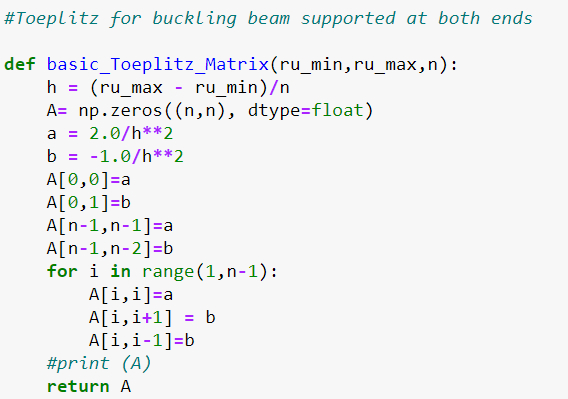
\includegraphics[width=\linewidth]{toeplitzbuckbeam.png}
  \caption{Toeplitz matrix for buckling beam supported at both ends}
  \label{fig:jacobialg}
\end{figure}


\begin{figure}[H]
  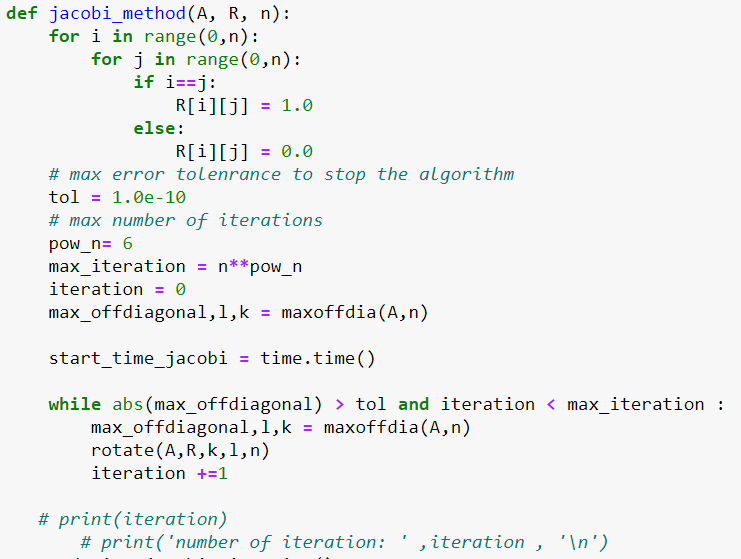
\includegraphics[width=\linewidth]{jacobialg.png}
  \caption{Jacobis rotation algorithm}
  \label{fig:jacobialg}
\end{figure}

\subsection{adaptation for Schrödinger equation for one electron}
The jacobi rotation algorithm is further extended to solve the \SL equation for one electron with only adaptation to set the Toeplitz Matrix 
The matrix is set as follows:


\begin{equation}
    \begin{bmatrix} \dfrac{2}{h^2}+V_1& \dfrac{-1}{h^2} & 0   & 0    & \dots  &0     & 0 \\
                                \dfrac{-1}{h^2} & \dfrac{2}{h^2}+V_2 & \dfrac{-1}{h^2} & 0    & \dots  &0     &0 \\
                                0   & \dfrac{-1}{h^2} & \dfrac{2}{h^2}+V_3 & \dfrac{-1}{h^2}  &0       &\dots & 0\\
                                \dots  & \dots & \dots & \dots  &\dots      &\dots & \dots\\
                                0   & \dots & \dots & \dots  &\dfrac{-1}{h^2}  &\dfrac{2}{h^2}+V_{nstep-2} & \dfrac{-1}{h^2}\\
                                0   & \dots & \dots & \dots  &\dots       & & \dfrac{2}{h^2}+V_{nstep-1}\end{bmatrix}
\label{eq:sc1matrixse}
\end{equation}
                            
\begin{figure}[H]
 	 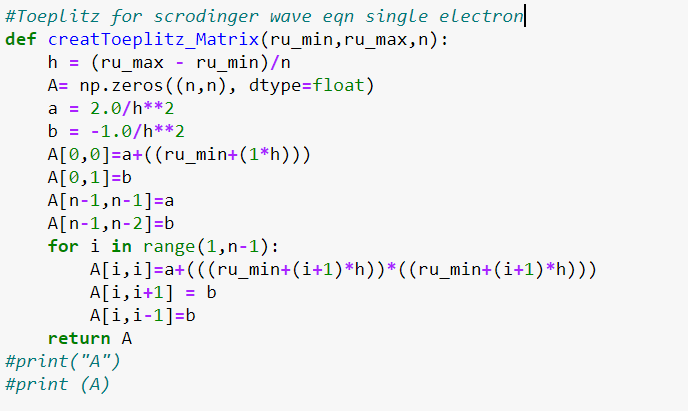
\includegraphics[width=\linewidth]{toeplitzscrodingersingleelec.png}
	\caption{Toeplitz Matrix for scrodinger equation for single electron}
  \label{fig:schro}
\end{figure}

The Jacobi eigenvalue method repeatedly performs rotation until the matrix becomes almost diagonal. Then
the diagonal elements are approximations of the eigenvalues of $S$.

\section{Results and Discussion}
Jacobi's rotation algorithm is studied for different Rho-max values and for different discretisation values and the results are given as below:
\begin{figure}[H]
 	 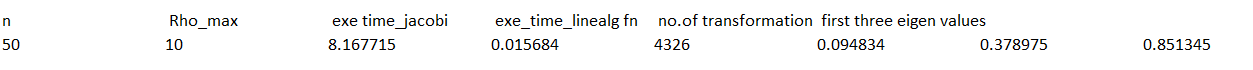
\includegraphics[width=\linewidth]{buckbeamtime.png}
	\caption{Jacobi's algorithm results for buckling beam problem  - n 50 and Rho-max 10}
  \label{fig:results for buckling beam problem}
\end{figure}

\begin{figure}[H]
 	 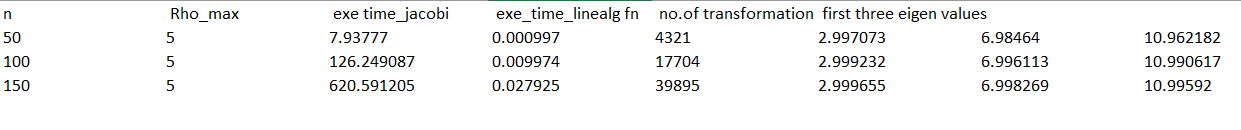
\includegraphics[width=\linewidth]{timerhomax5n150.png}
	\caption{Jacobi's algorithm results for scrodinger equation for single electron - n til 150 and Rho-max 5}
  \label{fig:results for buckling beam problem}
\end{figure}

\begin{figure}[H]
 	 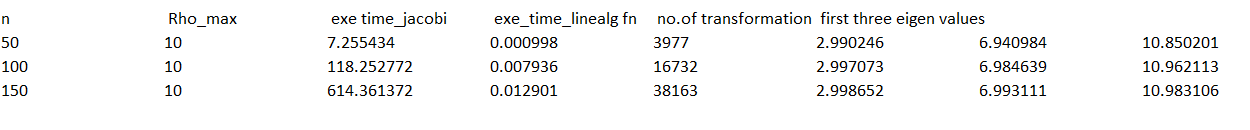
\includegraphics[width=\linewidth]{timerhomax10n150.png}
	\caption{Jacobi's algorithm results for scrodinger equation for single electron - n til 150 and Rho-max 10}
  \label{fig:schro}
\end{figure}

The results are provided under project 2 of git repositary.

Jacobi's rotation method is implemented to find eigen values for the bucking beam problem and found to be same with the analytical solution.Similarly  \SL equation for one electron is solved for the eigenvalues and found to be same as of built in Numpy function linalg.eig
it is observed that for getting first three eigen values close to the approximation of 4 digits , number og discretion points should be at least n $=$200 at Rho-max is 10. 
Even though Jacobi's rotation algorithm gives correct solutions , it consumes lot of time as shown , hence practically not usable for n $>$ 250 .Parallelisation techniques can be used to speed up the execution of the algorithm to certain extend.
So other efficient algorithms as Lanzcos algorithm need to be studied and used . 

\section{Unit Test}
In this section i have implemented a unit test for the buckling beam problem using Jacobi's rotation algorithm as follows and the results are found to be same as from numpy fucntion

\begin{figure}[H]
 	 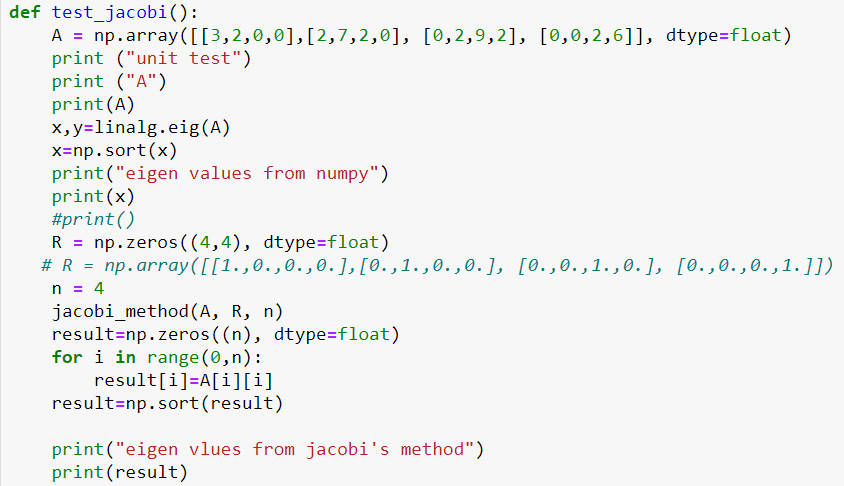
\includegraphics[width=\linewidth]{unittestbuckbeam.png}
	\caption{ unit test for Jacobi's algorithm -buckling beam problem}
  \label{fig:unit test  }
\end{figure}

\begin{figure}[H]
 	 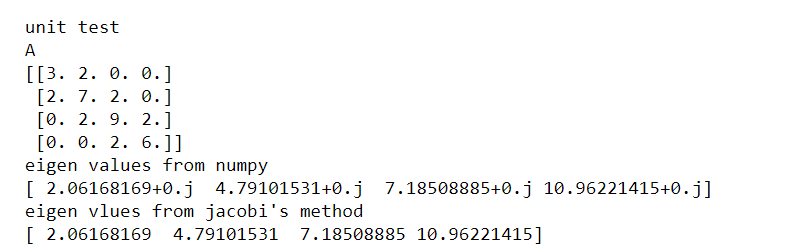
\includegraphics[width=\linewidth]{unittestresult.png}
	\caption{  Result of unit test for Jacobi's algorithm -buckling beam problem}
  \label{fig:Result of unit test for Jacobi's algorithm -buckling beam problem }
\end{figure}

\section{Conclusion}
The Jacobi rotation method or eigen value problem is very slow method to find eigenvalues compared to the built in method  in the python \texttt{numpy} library.
 For systems where a relatively small number of grid points $n$ is sufficient, the Jacobi method may be the preferred method. 


\end{document} 
